\documentclass[landscape]{beamer}

\mode<handout>
{
  \usepackage{pgf}
  \usepackage{pgfpages}

\pgfpagesdeclarelayout{6 on 1 boxed}
{
  \edef\pgfpageoptionheight{\the\paperheight} 
  \edef\pgfpageoptionwidth{\the\paperwidth}
  \edef\pgfpageoptionborder{0pt}
}
{
  \pgfpagesphysicalpageoptions
  {%
    logical pages=6,%
    physical height=\pgfpageoptionheight,%
    physical width=\pgfpageoptionwidth%
  }
  \pgfpageslogicalpageoptions{1}
  {%
    border code=\pgfsetlinewidth{2pt}\pgfstroke,%
    border shrink=\pgfpageoptionborder,%
    resized width=.5\pgfphysicalwidth,%
    resized height=.5\pgfphysicalheight,%
    center=\pgfpoint{.25\pgfphysicalwidth}{.833\pgfphysicalheight}%
  }%
  \pgfpageslogicalpageoptions{2}
  {%
    border code=\pgfsetlinewidth{2pt}\pgfstroke,%
    border shrink=\pgfpageoptionborder,%
    resized width=.5\pgfphysicalwidth,%
    resized height=.5\pgfphysicalheight,%
    center=\pgfpoint{.75\pgfphysicalwidth}{.833\pgfphysicalheight}%
  }%
  \pgfpageslogicalpageoptions{3}
  {%
    border code=\pgfsetlinewidth{2pt}\pgfstroke,%
    border shrink=\pgfpageoptionborder,%
    resized width=.5\pgfphysicalwidth,%
    resized height=.5\pgfphysicalheight,%
    center=\pgfpoint{.25\pgfphysicalwidth}{.5\pgfphysicalheight}%
  }%
  \pgfpageslogicalpageoptions{4}
  {%
    border code=\pgfsetlinewidth{2pt}\pgfstroke,%
    border shrink=\pgfpageoptionborder,%
    resized width=.5\pgfphysicalwidth,%
    resized height=.5\pgfphysicalheight,%
    center=\pgfpoint{.75\pgfphysicalwidth}{.5\pgfphysicalheight}%
  }%
  \pgfpageslogicalpageoptions{5}
  {%
    border code=\pgfsetlinewidth{2pt}\pgfstroke,%
    border shrink=\pgfpageoptionborder,%
    resized width=.5\pgfphysicalwidth,%
    resized height=.5\pgfphysicalheight,%
    center=\pgfpoint{.25\pgfphysicalwidth}{.167\pgfphysicalheight}%
  }%
  \pgfpageslogicalpageoptions{6}
  {%
    border code=\pgfsetlinewidth{2pt}\pgfstroke,%
    border shrink=\pgfpageoptionborder,%
    resized width=.5\pgfphysicalwidth,%
    resized height=.5\pgfphysicalheight,%
    center=\pgfpoint{.75\pgfphysicalwidth}{.167\pgfphysicalheight}%
  }%
}


  \pgfpagesuselayout{6 on 1 boxed}[letterpaper, border shrink=5mm]
  \nofiles
}

%\usetheme{Antibes}
%\usetheme[compress]{Singapore}
\usetheme{Warsaw} 
\usecolortheme{default}

\hypersetup{pdfpagemode=FullScreen}

%\definecolor{amber}{rgb}{1.0, 0.75, 0.0}
%\definecolor{alizarin}{rgb}{0.39, 0.58, 0.93}
%\setbeamercolor{structure}{fg=amber!85!black}
\usefonttheme[onlymath]{serif}
%\setbeamercovered{transparent}

\usepackage[T1]{fontenc}
\usepackage{colortbl}
\usepackage{multimedia}
\usepackage{graphicx}
\usepackage{lmodern, textcomp}
\usepackage{multicol}
\usepackage{comment}
\setlength{\columnsep}{1cm}
\usepackage{xcolor}
\usepackage{tikz,tkz-euclide}
\usetikzlibrary{calc}
\usetikzlibrary{decorations.pathreplacing}
\usetikzlibrary{shapes.misc, positioning}
\tikzset{vertex/.style={circle, fill=black, draw=black, inner sep=0pt, minimum size=1.15ex}}
%%%%%%%%%%%%%%%%%%%%%%%%%%%%%%%%%%%%%%%%

\usepackage{graphicx}  % Required for including images
\graphicspath{{./images/}}

\newcommand{\Z}{\ensuremath{Z}}
\newcommand{\K}[1][3]{\ensuremath{K^{(#1)}}}
\let\Lstroke=\L
\renewcommand{\L}[1][3]{\ensuremath{L^{(#1)}}}
\newcommand\multiset[2][\lambda]{\vphantom{#2}^{#1\!}#2}
\let\ms=\multiset

\newtheorem{maintheorem}{Main Theorem}

\definecolor{darkgreen}{rgb}{0,0.39,0}
\definecolor{darkred}{rgb}{0.5,0.1,0.1}
%\colorlet{mygold}{amber!85!black}

\newcommand\drawHedge[4][]{\draw [thick, #1] (#2) edge[bend left] (#3) edge (#4) (#3) edge (#4);}
%%%%%%%%%%%%%%%%%%%%%%%%%%%%%%%%%%%%%%%%

\title[Grates]{All the Right ``Grates''}

%\author[Lariccia] {Zachary~Lariccia,.\texorpdfstring{\rlap,}*\\
%\vspace{1em}
%Southern Connecticut State University}
\author[Lariccia] {Zachary~Lariccia}
\institute[CCSU]{Central Connecticut State University\\}
% \medskip
% (Joint work with Brian Darrow, Joe Fields, Heiko Todt)}

\date[CCSU Spring 2025] {Mathematics Department Colloquium \\[1em]
\small Central Connecticut State University \\
\small New Britain, CT\\
\small October 31, 2025}

% \newcommand\grantNumber{A1950357}
% \newcommand\grantTitle{REU\slash RET Site: Mathematics Research Experience \\ for Pre-Service and for In-Service Teachers and Students}


%%%%%%%%%%%%%%%%%%%%%%%%%%%%%%%%%%%%%%%%

\begin{document}

\maketitle
\section{Abstract}
    \begin{frame}{Abstract}
        \includegraphics[width=1.00\linewidth]{Abstract.png}
    \end{frame}



\section{Introduction to the $1$-Dimensional Problem}

        { %magic to get a full screen image...
        \setbeamertemplate{navigation symbols}{}  % hide navigation buttons
        \setbeamertemplate{background canvas}{\centerline{\includegraphics
        [height=\paperheight]{grade_sheet.JPG}}}
        \begin{frame}{Ever Been in this Situation?}
            \rule{0pt}{0pt}
        \end{frame}

    } %end of magic

            { %magic to get a full screen image...
        \setbeamertemplate{navigation symbols}{}  % hide navigation buttons
        \setbeamertemplate{background canvas}{\centerline{\includegraphics
        [height=\paperheight]{actual_grate.JPG}}}
        \begin{frame}[plain]
            \rule{0pt}{0pt}
        \end{frame}

    } %end of magic

        \begin{frame}{Grate Expectations}
        \begin{center}
            \includegraphics[scale=2]{DickensCover.pdf}
        \end{center}
    \end{frame}


    \begin{frame}{Grate Expectations}
        \transfade
        \begin{center}
            \includegraphics[scale=2]{DickensCover_Grate_2.jpg}
        \end{center}
    \end{frame}


    \begin{frame}{Grate Beginnings}
        \begin{itemize} \addtolength\itemsep{1em}
        \item Dr. Joe Fields (SCSU) first encountered the problem years ago while recording grades
        \item Dr. Fields shared the problem with Dr. Darrow, which began their ``grate" work
        \end{itemize}
    \end{frame}


    \begin{frame}{The Original ``Grate" Problem}
        \begin{itemize} \addtolength\itemsep{1em}
        \item In recording scores by hand, a great deal of care is needed--until it's not.
        \item When you've entered enough grades so that only isolated cells, blank positions with no other blank positions adjacent to them, remain.
        \item We refer to such an arrangement as a \textit{grate}.
        \end{itemize}
    \end{frame}

    \begin{frame}{The Grate Problem}
        \begin{itemize} \addtolength\itemsep{1em}
        \item The problem that emerged is: What is the expected number of scores recorded before we will have a grate?
        \item There are some trivial bounds on this expected value.
        \end{itemize}
    \end{frame}


\begin{frame}{Some Grate Bounds}
\begin{itemize} \addtolength\itemsep{1em}
  \item If $n-1$ scores have been recorded, you certainly have a grate!
  \item If $n-2$ scores have been recorded, you \textit{usually} have a grate.
  \item If fewer than $\lfloor\frac{n}{2}\rfloor$ scores have been recorded, you certainly do not have a grate.
\end{itemize}
\end{frame}


\begin{frame}{Grate Abstractions}
\begin{itemize} \addtolength\itemsep{1em}
  \item Consider a permutation $\pi$ of $\{1, 2, 3, \ldots , n\}$.  
  \item Beginning with a vector of length $n$ consisting of all $0$s, consider the following $n$-step procedure: For $i$ from $1$ to $n$ turn the zero in position $\pi(i)$ into a $1$.  A grate (in this context) is a binary vector having only isolated zeros.  Let $f(\pi)=k$ if at stage $k$ we have a grate but at stage $k-1$ we do not.  Assuming all permutations are equally likely, we have

\[ E = \frac{1}{n!} \sum_{\pi \in S_n} f(\pi) \]
\end{itemize}
\end{frame}

% \begin{frame}{What is a 1-D grate}
% \begin{itemize}\addtolength\itemsep{0.8em}
%   \item A 1-D grate is a length-$n$ 0--1 string with no consecutive zeros.
%   \item Notation: $G(n,k)$ for the set, $g(n,k)=|G(n,k)|$.
%   \item \emph ``Only isolated 0s'' means the substring ``00'' is forbidden while fixing the number of ones $k$.
%   \item $01101101$ is a valid 1-dimensional grate of length $8$ with $5 (k)$ ones.
%   \item $11101001$ is NOT a valid 1-dimensional grate of length $8$ with $5 (k)$ ones.
% \end{itemize}
% \end{frame}


        \begin{frame}{Small Examples}
        \begin{table}[htbp]
            \begin{tabular}{|r||c|c|c|c|c|c|} \hline
            & $k=1$ & 2 & 3 & 4 & 5 & 6 \\ \hline\hline
            $n=1$   & 1     &       &       &       &       & \\[8pt] \hline
%
            $2$     & 10    & 11    &       &       &       & \\
            & 01    &       &       &       &       & \\[8pt] \hline
%
            $3$     & 010   &  011  & 111   &       &       & \\
            &       &  101  &       &       &       & \\
            &       &  110  &       &       &       & \\[8pt] \hline
%
            $4$     &       & 0101  & 0111  & 1111  &       & \\
            &       & 1010  & 1011  &       &       & \\
            &       & 0110  & 1101  &       &       & \\
            &       &       & 1110  &       &       & \\[8pt] \hline
            \end{tabular}
        \end{table}
    \end{frame}


    \begin{frame}{Grate Possibilities}
        \begin{table}[htbp]
            \begin{tabular}{|r||c|c|c|c|c|c|} \hline
            & $k=1$ & 2 & 3 & 4 & 5 & 6 \\ \hline\hline
            $5$     &       & 01010 & 01011 & 01111 & 11111 & \\
            &       &       & 10101 & 10111 &       & \\
            &       &       & 01101 & 11011 &       & \\
            &       &       & 01110 & 11101 &       & \\
            &       &       & 10110 & 11110 &       & \\
            &       &       & 11010 &       &       & \\[8pt] \hline
            \end{tabular}
        \end{table}
    \end{frame}

    \begin{frame}{Grate Possibilities}
        \begin{table}[htbp]
            \begin{tabular}{|r||c|c|c|c|c|c|} \hline
            & $k=1$ & 2 & 3 & 4 & 5 & 6 \\ \hline\hline
%
            $6$     &       &       & 010110& 010111 & 011111 & 111111 \\
            &       &       & 101010& 101011 & 101111 &       \\
            &       &       & 011010& 011011 & 110111 &       \\
            &       &       & 010101& 011101 & 111011 &        \\
            &       &       &       & 101101 & 111101 &        \\
            &       &       &       & 110101 & 111110 &       \\
            &       &       &       & 011110 &        & \\
            &       &       &       & 101110 &        & \\
            &       &       &       & 110110 &        & \\
            &       &       &       & 111010 &        & \\[8pt] \hline
            \end{tabular}
        \end{table}
    \end{frame}

        \begin{frame}{A Grate Recursion}
        \begin{itemize} \addtolength\itemsep{1em}
        \item We started by counting up the number of possible grates for small values of $n$ and $k$.
        \item Eventually, we found a recursive approach to listing all the grates of a given length.
        \item After too, too much time\dots
        \item Of course! Pascal's Triangle!
        \end{itemize}
    \end{frame}

    \begin{frame}{The Grate Pascal's Triangle}
        \begin{table}[htbp]
            \begin{tabular}{|r||c|c|c|c|c|c|} \hline
            & $k=1$ & 2 & 3 & 4 & 5 & 6 \\ \hline\hline
            $n=1$  & 1    &      &       &       &       &   \\[8pt] \hline
            $2$     & 2   &  1   &       &       &       &   \\[8pt] \hline
            $3$     & 1   &  3   &   1   &       &       &   \\[8pt] \hline
            $4$     &     &  3   &   4   &    1  &       &   \\[8pt] \hline
            $5$     &     &  1   &   6   &    5  &     1 &   \\[8pt] \hline
            $6$     &     &      &   4   &   10  &     6 & 1 \\[8pt] \hline
            \end{tabular}
        \end{table}
    \end{frame}

        \begin{frame}{Our First Grate Theorem}
        \begin{itemize} \addtolength\itemsep{1em}
        \item Let $g(n,k)$ denote the number of grates with length $n$ and $k$ ones. The recursion for binomial coefficients, and the shifting of the entries in Pascal's Triangle within the table, led us to prove that

        \[g(n,k)=g(n-1,k-1)+g(n-2,k-1)\]

        \item Note that $G(n,k)$ denotes the set of grates that exist for a given $n$ and $k$, while $g(n,k)=|G(n,k)|$
        \end{itemize}
    \end{frame}

    

        \begin{frame}{Another Grate Theorem and Proof }
        \begin{theorem}
            The number of bitstrings of length $n$ with $k$ 1s and only isolated 0s is $\binom{k+1}{n-k}$.
        \end{theorem}

        \begin{Proof}
            Consider a length $k$ bitstring containing all $1$'s.  There are $k+1$ positions before, after, or between these $1$'s. Then, select $n-k$ of those positions to insert the (individual) $0$'s.
        \end{Proof}

    \end{frame}

        \begin{frame}{Some Grate Geometry}
        \begin{itemize} \addtolength\itemsep{1em}
        \item One way to think about this problem is to imagine the $n$-hypercube, with the origin $\vec{0}$ representing the all-zeroes vector, and $\vec{1}$ representing the all-ones vector.
        \item There are two parameters for a grate, the length $n$ and the number of ones, $k$ (which can be thought of as having weight $k$).
        \item We would then be concerned with the increasing paths from the bottom ($\vec{0}$) to the top ($\vec{1}$) of the $n$-hypercube (as a graded poset) which first encounter a grate at stage $k$, weighted by $k$.
        \item Of particular importance are what we call ``transition edges'', or those connecting a non-grate to a grate.
        \end{itemize}
    \end{frame}

            \begin{frame}{Hypercube}
            \includegraphics[width=0.8\linewidth]{Hypercube(n=5).png}
    \end{frame}

        \begin{frame}{Shifting the Focus to Grate Path Counting}
        \begin{itemize} \addtolength\itemsep{1em}
        \item Recall that we can think about this problem in terms of paths in the $n$-hypercube, $Q_n$.
        \item A ``path'' in $Q_n$ starts at $\vec{0}$, ends at $\vec{1}$, and always moving increasingly up the grade.
        \item All paths begin at a non-grate (unless $n=1$) and eventually pass into a grate.  Once a path has reached a node that is a grate, it will remain amongst the grates from that point onward.
        \item We're interested in counting the paths that first reach a grate after $k$ steps. In other words we want to count the paths that are at a non-grate at stage $k-1$ and hit a grate at stage $k$.
        \end{itemize}
    \end{frame}

    \begin{frame}{Grate Layers}
        \begin{center}
            \includegraphics[scale=.4]{GratePIC.PNG}
            % \input{grate_layers.pdf_t}
        \end{center}
    \end{frame}


        \begin{frame}{Grate Permanence}
        \begin{itemize} \addtolength\itemsep{1em}
        \item Once you're a grate, you're always a grate
        \item This leads us to counting the edges that transition a non-grate to a grate
        \item Transition edges (going from level $k-1$ to level $k$):

        \[ \left[ k \binom{k+1}{n-k} - (n-k+1) \binom{k}{n-k+1} \right] \]

        \end{itemize}
    \end{frame}

    
        \begin{frame}{Grate Expectations}
        \begin{itemize} \addtolength\itemsep{1em}
        \item From this, we get the formula for the expectation:

        \[ \frac{1}{n!} \cdot \sum_{k=1}^n k \cdot p(n,k). \]

        \item Taking note of the fact that $p(n,n) = 0$, and that $p(n,k) = 0$ whenever $k < \lfloor n/2 \rfloor$, this becomes

        \[ \frac{1}{n!} \cdot \sum_{k=\lfloor n/2 \rfloor}^{n-1} k \cdot \left[ \binom{k+1}{n-k} - \binom{k-1}{n-k} \right] \cdot (k)! \cdot (n-k)! \]

        \noindent
        \end{itemize}
    \end{frame}

    \begin{frame}{A Visually Grate Final Formula}
    \begin{itemize}
        \item Or in a more visually grate form (hence a separate slide)...
        \medskip
        \medskip

        \[\huge{\sum_{k=\lfloor n/2 \rfloor}^{n-1} k \cdot  \frac{\binom{k+1}{n-k} - \binom{k-1}{n-k}}{\binom{n}{k}} } \]

    \end{itemize}
    \end{frame}

%        \begin{frame}{First Pascal \dots Now Fibonacci?! How Grate!}
%        \begin{itemize} \addtolength\itemsep{1em}
%        \item The count of the transition edges is actually a sequence in OEIS,  A067331.
%        \item The entry was ``Convolution of Fibonacci $F(n+1)$, $n\geq 0$, with $F(n+3)$, $n\geq 0$.''
%        \item This was rather, let's say, ``unenlightening.''
%        \item More investigation led to the discovery of Fibbinary numbers, which are just a bit-flip away from grates (not the expectation, however!)
%        \end{itemize}
%    \end{frame}

\begin{frame}{First Pascal \dots Now Fibonacci?! How Grate!}
\begin{itemize} \addtolength\itemsep{1em}
        \item The count of the transition edges is actually a sequence in OEIS,  A067331.
        \item More investigation led to the discovery of Fibbinary numbers, which are just a bit-flip away from grates (not the expectation, however!)
        \end{itemize}
\begin{theorem}
    $\displaystyle \forall n \in {\mathbb Z}^+, \; \sum_{k=\lfloor n/2 \rfloor}^n g(n,k) \; = \; F_{n+1}.$  Where $F_n$ denotes the $n$th Fibonacci number.
\end{theorem}
\end{frame}

    \section{The Talk}

\begin{frame}{A ``Grate" Inspiration}
  \centering The day I attended a ``grate" talk...
\end{frame}

\begin{frame}{My Story}
\begin{itemize}\addtolength\itemsep{0.8em}
  \item I was enrolled in Dr. Darrow's Calculus 1 class at CCSU in Fall 2024, where he mentioned his upcoming colloquium talk
  \item I attended and was instantly intrigued by the problem and knew I could contribute
  \item Less than two weeks later, I was in Dr. Darrow's office showing him output from programs I developed to investigate higher dimensional grates
\end{itemize}
\end{frame}

\begin{frame}{Grate Drafts!}
  \textbf{1st Drafts}\\[0.4em]
  \includegraphics[width=\linewidth,height=1.0\textheight,keepaspectratio]{draft_grates.jpg}
\end{frame}

\begin{frame}{Two-Dimensional Grate Definitions}
\begin{itemize}\addtolength\itemsep{0.8em}
  \item In $1$-dimensional grates, there are no two adjacent zeroes in a binary bitstring.
  \item In $2$-dimensions, one can define a grate in several ways
  \item The most natural to us was defining a grate as a two-dimensional array where each $0$ is completely isolated on all sides (8 neighboring directions)
  \item That is,for any given $0$ in the array, there are no other zeroes above, below, to the left, to the right, diagonally, or antidiagonally
  \item We call these ``full grates"
\end{itemize}
\end{frame}

\begin{frame}{$2\times n$ Full Grate Examples}
\begin{columns}[T,onlytextwidth]
  \column{0.48\textwidth}
  \textbf{Full Grate $2\times 5$ ($8$) Ones}\\[0.4em]
  \includegraphics[width=\linewidth,height=0.62\textheight,keepaspectratio]{2x5_8ones.png}

  \column{0.48\textwidth}
  \textbf{Full Grate $2 \times 10$ ($15$) Ones}\\[0.4em]
  \includegraphics[width=\linewidth,height=0.62\textheight,keepaspectratio]{2x10_15ones.png}
\end{columns}
\end{frame}

\begin{frame}{$3\times 3$ Full Grates}
\begin{columns}[T,onlytextwidth]
  \column{0.48\textwidth}
  \textbf{Full Grate}\\[0.4em]
  \includegraphics[width=\linewidth,height=0.62\textheight,keepaspectratio]{full-grate.png}

  \column{0.48\textwidth}
  \textbf{Not a Full Grate}\\[0.4em]
  \includegraphics[width=\linewidth,height=0.62\textheight,keepaspectratio]{not-a-full-grate.png}
\end{columns}
\end{frame}

% \begin{frame}{A Grate Problem: how a tiny rule led to big patterns}
% \begin{itemize}\addtolength\itemsep{0.8em}
%   \item We study 0--1 patterns where ``holes on a grade sheet'' (zeros in matrices) follow a simple isolation rule.
%   \item Start in 1-D, then extend to 2-D and variants.
%   \item \emph View patterns as constrained bitstrings and grid graphs, later as regions and paths in the graded Darrow hypercube.
% \end{itemize}
% \end{frame}

% \begin{frame}{Glossary}
%     \small
%     \begin{tabular}{p{0.28\textwidth} p{0.72\textwidth}}
%         \textbf{Full grate} & A grid with only isolated zeros in all 8 neighborhood directions. \emph{Advanced:} independent set in king's graph. \\[0.8em]

%         \textbf{Mask} & Column masks in dynamic programming (DP) refer to using bitmask representations for subsets of columns or states in grid problems, allowing efficient tracking and transitions. \\[0.8em]

%         \textbf{Compatibility} & Two masks can sit side by side. \emph{Advanced:} forbid horizontal and diagonal zero neighbors. \\[0.8em]

%         \textbf{BigInteger} & Java type for large totals. \emph{Advanced:} arbitrary precision integers. \\[0.8em]

%         \textbf{8-neighborhood} & All adjacent and diagonal neighbors. \emph{Advanced:} king moves on a chessboard. \\[0.8em]

%         \textbf{Enumeration} & Try all placements. \emph{Advanced:} choose $k$ of $mn$ cells and backtrack. \\
%     \end{tabular}
% \end{frame}


\begin{frame}{Other Definitions}
\begin{itemize}\addtolength\itemsep{0.8em}
  \item The ``plus-sign" grate, where zeroes in the array are not adjacent to another above, below, to the left, and to the right 
  \item The ``$X$"-grate, where zeroes in the array are not adjacent diagonally or anti-diagonally.
\end{itemize}
\end{frame}

\begin{frame}{Plus and X Grates}
\centering
\begin{minipage}{0.48\linewidth}
    \centering
    \includegraphics[width=\linewidth]{3x3Plus.png}
    \captionof{Plus Grate }{$3 \times 3$ ($4$ ones)}
    \label{fig:counter}
\end{minipage}\hfill
\begin{minipage}{0.48\linewidth}
    \centering
    \includegraphics[width=\linewidth]{4x5(9_ones)XGrate.png}
    \captionof{X Grate }{$4 \times 5$ ($9$ ones)}
    \label{fig:visualizer}
\end{minipage}
\end{frame}




% \begin{frame}{What is a 2-D grate?}
% \begin{itemize}\addtolength\itemsep{0.8em}
%   \item We consider a 2-dimensional array such that no 0 is adjacent to any other above, below, to the right, to the left, diagonally, or anti-diagonally. 

%   \item We have called these “full” grates, full being a full grate isolation rule of the 8-Neighbors.
%   \item $n \times n$ for nonnegative values $n$.
%   \item $m \times n$ rectangular binary arrays, the length and height of the array, respectively.
%   \item We can count by fixed ones $k$ or totals.
% \end{itemize}
% \end{frame}



% \begin{frame}{First experiments: list small cases and spot a pattern}
% \begin{itemize}\addtolength\itemsep{0.8em}
%   \item Start by listing all valid strings for small $n,k$ (brute force).
%   \item A shifted Pascal structure emerges for $g(n,k)$.
%   \item \emph Grate Counting Recursion! $g(n,k)=g(n\!-\!1,k\!-\!1)+g(n\!-\!2,k\!-\!1)$.
% \end{itemize}
% \end{frame}

% \begin{frame}{The clean counting formula: a choose-argument}
% \begin{itemize}\addtolength\itemsep{0.8em}
%   \item Start with $k$ ones, choose the $n-k$ gap positions to place zeros.
%   \item Result: $g(n,k)=\binom{k+1}{\,n-k\,}$.
%   \item \emph Choose among the $k\!+\!1$ slots before, after, or between ones.
% \end{itemize}
% \end{frame}

% \begin{frame}{A Fibonacci surprise: summing across $k$}
% \begin{itemize}\addtolength\itemsep{0.8em}
%   \item Summing grates across valid $k$ gives a Fibonacci number.
%   \item \emph {$\sum_{k=\lfloor n/2\rfloor}^{n} g(n,k)=F_{n+1}$ with a reversible end-bit argument.}
% \end{itemize}
% \end{frame}

\begin{frame}{The Dream Team}
\begin{itemize}\addtolength\itemsep{0.8em}
  \item Dr. Darrow and Dr. Fields brute-force 1-D tables led to patterns, then proofs, and my software formulated conclusions for 2-D which would've been extensive doing by hand.
  \item These programs allowed us to count up, and visualize, all the $m\times n$ full, plus, and x-grates for reasonably large values of inputs; the team extended to 2-D and expectations.
  \item I built a total of 17 custom tailored programs (visualizers and counters)
\end{itemize}
\end{frame}

\begin{frame}{Grate Projects Overview}
\vspace{-0.8em}
\textbf{Sorted by Dimension:}

\begin{columns}
  \column{0.48\textwidth}
    \textbf{\footnotesize m $\times$ n Type}
    \begin{itemize}\footnotesize
      \setlength{\itemsep}{1pt}
      \item mxn-X-Grate-Counter-Optimized
      \item mxn-X-Grate-Visualizer
      \item mxn-Full-Grate-Counter
      \item mxn-Full-Grate-Counter-Optimized
      \item mxn-Full-Grate-Visualizer
      \item mxn-Plus-Grate-Counter
      \item mxn-Plus-Grate-Counter-Optimized
      \item mxn-Plus-Grate-Counter-Reformatted
      \item mxn-Plus-Grate-Visualizer
    \end{itemize}

  \column{0.48\textwidth}
    \textbf{\footnotesize n $\times$ n Type}
    \begin{itemize}\footnotesize
      \setlength{\itemsep}{1pt}
      \item nxn-Full-Grate-Counter
      \item nxn-Full-Grate-Determinant
      \item nxn-Full-Grate-Visualizer
      \item nxn-Plus-Grate-Counter
      \item nxn-Plus-Grate-Counter-Reformatted
      \item nxn-Plus-Grate-Visualizer
      \item nxn-X-Grate-Counter
      \item nxn-X-Grate-Visualizer
    \end{itemize}
\end{columns}
\vspace{-0.5em}
\end{frame}

\begin{frame}{The Dream Team pt. 2}
\begin{itemize}\addtolength\itemsep{0.8em}
\item In comes Dr. Heiko Todt, a mathematician and a close colleague of both Dr. Fields and Dr. Darrow.
  \item After analyzing the output with Dr. Darrow, Dr. Todt then led an expedition to extend the expectation work to two-dimensional arrays
  \item Dr. Todt spent a while looking at 2xn versions of the full grates, as they held significance with a famous mathematical integer sequence
  \item We determined that the count of all possible $2\times n$ full grates yields the sequence of the Jacobthsal numbers
  \item These seemed like the most natural to begin extending the work from the 1-dimensional grates and the expectation.
\end{itemize}
\end{frame}


\section{From Lines to Boards}

    \begin{frame}{What is a DP (Dynamic Programming)}
        \small
        \begin{block}{Dynamic Programming}
            Dynamic programming is an algorithmic technique for solving optimization problems
            by breaking them down into smaller, overlapping subproblems.
        \end{block}

        \begin{exampleblock}{In the context of "Grates"}
            A way to count all legal grates by building them one row at a time and reusing partial results,
            instead of rechecking the same work repeatedly.
        \end{exampleblock}

        \begin{alertblock}{Why this matters}
            It tracks only the information that matters for the next step (the last row),
            which collapses an exponential search into something manageable.
        \end{alertblock}
    \end{frame}

    \begin{frame}{How to think about the software}
        \begin{itemize}\addtolength\itemsep{0.8em}
        \item A \textit{recipe}: precise steps that guarantee the grate rule is respected.
        \item A \textit{toolkit}: The counter for big enumeration, The visualizer for concrete and specific examples.
        \item A \textit{safety checker}: local rules prevent forbidden neighbor pairs and optimized version of the original algorithm.
        \end{itemize}
    \end{frame}

        \begin{frame}{Why this matters}
        \begin{itemize}\addtolength\itemsep{0.8em}
        \item Rules and patterns make fragile systems robust - like spacing holes so a grate stays strong.
        \item Software lets us explore many cases quickly - beyond what we can do by hand.
        \item Visual feedback helps learners and researchers alike connect definitions to concrete examples.
        \end{itemize}
    \end{frame}

        \begin{frame}{Meet the two programs}
        \small
        \textbf{Full Grate Counter}\\
        \emph{Counts binary $m\times n$ matrices with isolated zeros via bitmask DP over compatible column masks.}

        \vspace{0.6em}
        \textbf{Full Grate Visualizer}\\
        \emph{Enumerates all possible grates where $m(length), n(width), k(ones)$, filters using a custom algorithm with an 8-neighbor isolation test, then renders with the ability to export the images.}
    \end{frame}

% ---------- Counter ----------
\begin{comment}
    \begin{frame}{Counter overview - FullGrateCounterGUI}
        \begin{itemize}\addtolength\itemsep{0.8em}
        \item Scan the grid column by column, only keep column patterns that play nicely with the previous column.
        \item Mini story: We ask ``How many safe layouts (valid grates) exist?'' and let the DP add up all legal paths through a compatibility graph.
        \item \emph{Independent sets on the king's graph over an $(m\times n)$ lattice (graph), counted by stepping through columns using a precomputed allowed-next-column table.}
        \end{itemize}
    \end{frame}
\end{comment}
\begin{comment}
    \begin{frame}{Counter: inputs and outputs}
        \begin{columns}[T]
            \begin{column}{0.48\textwidth}
                \textbf{Inputs}
                \begin{itemize}
                    \item Rows $m$ \quad Columns $n$
                \end{itemize}
            \end{column}
            \begin{column}{0.48\textwidth}
                \textbf{Outputs}
                \begin{itemize}
                    \item For each $k$, number of full grates with exactly $k$ ones
                    \item BigInteger totals shown in the GUI and optional file save
                \end{itemize}
            \end{column}
        \end{columns}
        \begin{itemize}
            \item \small\emph{DP tracks a count for each compatible column mask and a running total of how many zeros so far, then converts to counts by ones $k$.}
        \end{itemize}
    \end{frame}
\end{comment}

    \begin{frame}{Counter in 3 steps}
        \begin{enumerate}\addtolength\itemsep{0.6em}
        \item Generate all column masks of height $m$ that avoid vertical zero adjacency.
        \item Build a compatibility table \texttt{compat[i][j]} that forbids horizontal and diagonal zero adjacency.
        \item Run a DP across $n$ columns that aggregates ways by zeros used, then translate to counts by ones.
        \end{enumerate}
        \small\emph{Time roughly $O\!\left(n\cdot P^2 \cdot mn\right)$ where $P$ is the number of valid masks and $mn$ bounds the zero counter range. Space about $O(P\cdot mn)$.}
    \end{frame}

    \begin{frame}{Counter}
\centering
\includegraphics[width=0.55\linewidth]{4x3Example.png}
\captionof{figure}{$4 \times 3$ ($9$ ones) Counter}
\label{fig:counter}
\end{frame}

\begin{frame}{Zoomed in Counter}
\centering
\includegraphics[width=0.3\linewidth]{zoomed-in-full-grate-counter.png}
\captionof{figure}{$4 \times 3$ ($9$ ones) Counter}
\label{fig:counter}
\end{frame}

    \begin{frame}[fragile]{Counter: tiny Java snippet - DP transition}
        \small
        \centering
\includegraphics[width=0.70\linewidth]{counter-code.png}
\label{fig:code}
    \end{frame}

    \begin{frame}{Counter: what could go wrong (but didn't)}
        \begin{itemize}\addtolength\itemsep{0.8em}
        \item Invalid masks - solved by filtering masks with $(mask \& (mask \ll 1))==0$.
        \item Big numbers - solved with \texttt{BigInteger} throughout.
        \item Runtime and memory - mitigated by using only two DP layers and precomputed compatibility.
        \end{itemize}
    \end{frame}

    \begin{frame}{Mini demo storyboard - Counter}
        \begin{columns}
            \begin{column}{0.32\textwidth}
                \begin{block}{1) Choose size}
                    Enter $m,n$ then click \textit{Run}.
                \end{block}
            \end{column}
            \begin{column}{0.32\textwidth}
                \begin{block}{2) Compute}
                    DP builds counts per $k$.
                \end{block}
            \end{column}
            \begin{column}{0.32\textwidth}
                \begin{block}{3) Read count}
                    Totals shown in the GUI; save to file if desired.
                \end{block}
            \end{column}
        \end{columns}
        \includegraphics[width=0.90\linewidth]{Counter-Demo.png}
    \end{frame}

    \begin{frame}{Counter 20x50}
        \includegraphics[width=0.90\linewidth]{20x50full.png}
    \end{frame}

% ---------- Visualizer ----------
\begin{comment}
    \begin{frame}{Visualizer overview - FullGrateVisualizer}
        \begin{itemize}\addtolength\itemsep{0.8em}
        \item Pick $m,n,k$ then step through every valid full grate with exactly $k$ ones. Save images if you like.
        \item Mini story: Generate all candidate layouts, filter by the full grate rule, show them in a clean grid.
        \item \emph{Backtracking enumerates all possible grates where ${m,n, k}$ for placement of ones, then a local 8-neighbor test validates each matrix.}
        \end{itemize}
    \end{frame}
\end{comment}

\begin{comment}
    \begin{frame}{Visualizer: inputs and outputs}
        \begin{columns}[T]
            \begin{column}{0.48\textwidth}
                \textbf{Inputs}
                \begin{itemize}
                    \item Rows $m$ \quad Columns $n$ \quad Target ones $k$
                \end{itemize}
            \end{column}
            \begin{column}{0.48\textwidth}
                \textbf{Outputs}
                \begin{itemize}
                    \item A browsable list of valid full grates with $k$ ones
                    \item Controls: Previous, Next, Save current, Save all
                \end{itemize}
            \end{column}
        \end{columns}
        \small\emph{If no valid layouts exist for $(m,n,k)$ the program reports that condition to the user.}
    \end{frame}
\end{comment}

    \begin{frame}{Visualizer in 3 steps}
        \begin{enumerate}\addtolength\itemsep{0.6em}
        \item Systematically place $k$ ones on an $m\times n$ grid.
        \item Check that every zero is isolated in the 8-neighborhood.
        \item Display the matrix and allow navigation or saving to PNG.
        \end{enumerate}
        \begin{itemize}
            \item \small\emph{Per-matrix validation is $O(mn)$ since there are 8 constant neighbors per cell.}
        \end{itemize}
    \end{frame}

    \begin{frame}{Figure: Visualizer data flow}
        \centering\footnotesize
        \resizebox{\linewidth}{!}{%
            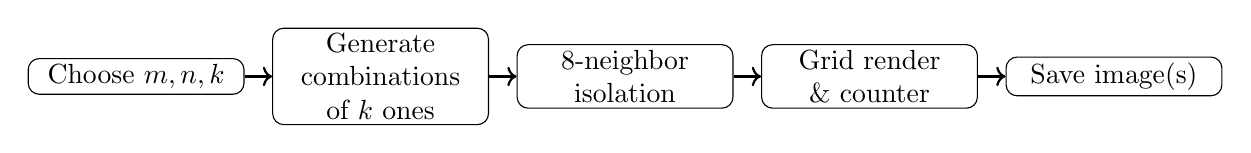
\begin{tikzpicture}[node distance=0.35cm,
                every node/.style={draw, rounded corners, align=center, inner sep=2pt, text width=2.6cm}]
                \node (pick) {Choose $m,n,k$};
                \node (gen)   [right=of pick]  {Generate combinations of $k$ ones};
                \node (check) [right=of gen]   {8-neighbor isolation};
                \node (view)  [right=of check] {Grid render\\\& counter};
                \node (save)  [right=of view]  {Save image(s)};
                \draw[->, thick] (pick) -- (gen);
                \draw[->, thick] (gen)  -- (check);
                \draw[->, thick] (check)-- (view);
                \draw[->, thick] (view) -- (save);
            \end{tikzpicture}}
        \includegraphics[width=0.70\linewidth]{5x4Full.png}
    \end{frame}

    \begin{frame}[fragile]{Visualizer: tiny Java snippet - full grate check}
        \includegraphics[width=1.05\linewidth]{VisualizerCode.png}
    \end{frame}

    \begin{frame}{Visualizer: what could go wrong again, but didn't}
        \begin{itemize}\addtolength\itemsep{0.8em}
        \item Large $mn$ and $k$ can make enumeration heavy - keep sizes modest or sample.
        \item Misclicks are not an issue in this viewer - navigation is by buttons with counts shown.
        \item Disk permissions when saving images - handled with standard file chooser and error dialogs.
        \end{itemize}
    \end{frame}

    \begin{frame}{Side-by-side comparison}
        \centering\footnotesize
        \resizebox{\linewidth}{!}{%
            \begin{tabular}{|l|c|c|}
                \hline
                & \textbf{Counter} & \textbf{Visualizer} \\\hline\hline
                Purpose & Count all valid layouts & Show valid layouts for fixed $k$ \\\hline
                Inputs & $m,n$ & $m,n,k$ \\\hline
                Core idea & DP over compatible masks & Enumerate and filter then render \\\hline
                Output & BigInteger counts by $k$ & Browse and save images \\\hline
                \emph{ & Transfer via $\mathrm{compat}[i][j]$ & 8-neighbor isolation test \\\hline}
            \end{tabular}}
    \end{frame}


\begin{frame}{Full Grate $2\times n$ Reformatted OEIS}
\includegraphics[width=1.3\linewidth,height=1.0\textheight,keepaspectratio]{OEIS_EXAMPLE.png}
\end{frame}

\begin{frame}{Non-Attacking Kings Connection}
\begin{itemize}\addtolength\itemsep{0.8em}
  \item The count of the full $n\times n$ grates correspond determining how many non-attacking kings can be placed on an $(n-1)\times(n-1)$ board.
\end{itemize}
\end{frame}

\begin{frame}{Non-Attacking Kings Example}
\centering
\begin{minipage}{0.48\linewidth}
    \includegraphics[width=\linewidth,keepaspectratio]{KING_MOVE.png}
\end{minipage}
\hfill
\begin{minipage}{0.48\linewidth}
    \includegraphics[width=\linewidth,keepaspectratio]{NONATTACKING_KINGS.png}
\end{minipage}
\end{frame}

\begin{frame}{Chessboard and Tilings Connection}
  \centering
  \textbf{OEIS A061995 (One of 700 Similiar Submissions on the Kings problem)}\\[0.6em]
  \includegraphics[width=1.0\linewidth,height=0.75\textheight,keepaspectratio]{kingsOEIS.png}
\end{frame}


\begin{frame}{Connection to Tiling Problems}
\begin{itemize}\addtolength\itemsep{0.8em}
  \item The counts of the number of $n\times n$ full grates is also the number of tilings of an $n\times n$ board by $1\times1$ and $2\times2$ tiles
\end{itemize}

\begin{center}
    \includegraphics[scale=.4]{11_2x2Tiles.png}
\end{center}
\end{frame}



\begin{frame}{Rectangular Grates: More Tiling Connections}
\begin{itemize}\addtolength\itemsep{0.8em}
  \item The number of full $m\times n$ grates equals tilings of an $(m\!+\!1)\times n$ rectangle by $1\times1$ and $2\times2$ blocks.
  \item A054855 - Number of ways to tile a $5 \times n$ area with $1 \times 1$ and $2 \times 2$ tiles. ($4 \times n$ for full grates)
  \item A063650 - Number of ways to tile a $6 \times n$ rectangle with $1 \times 1$ and $2 \times 2$ tiles. ($5 \times n$ for full grates)
\end{itemize}
\end{frame}

\begin{frame}{OEIS Entries for Plus and X-Sign Grates}
\begin{itemize}\addtolength\itemsep{0.8em}
  \item Both X-Sign and Plus-Sign Grates are also known as placing non-attacking bishops \& wazirs respectively.
  \item A181212 - $T(n,k)$=Number of $n \times k$ binary matrices with no two $1$'s adjacent diagonally or antidiagonally.
  \item A201511 - Number of ways to place $n$ nonattacking wazirs on an $n \times n$ board.
\end{itemize}
\end{frame}

\begin{frame}{Jacobsthal Connection}
\begin{itemize}\addtolength\itemsep{0.8em}
  \item Ernst Jacobsthal was a German mathematician known for his work in number theory and for the Jacobsthal numbers, which are an integer sequence named after him.
  \item A001045 - Jacobsthal sequence (or Jacobsthal numbers): a(n) = a(n-1) + 2*a(n-2), with a(0) = 0, a(1) = 1
  \item The general Jacobsthal Reccurence formula is \[ J_n = J_{n-1} + 2J_{n-2}, \quad J_0 = 0, \quad J_1 = 1 \]
  \item For $2\times n$, total of possible full grates are the Jacobsthal numbers.
\end{itemize}
\end{frame}




% \begin{frame}{Special families that pop: $2\times n$ and $3\times n$}
% \begin{itemize}\addtolength\itemsep{0.8em}
%   \item For $2\times n$, totals are the Jacobsthal numbers.
%   \item For $3\times n$, the triangle by ones $k$ matches OEIS A128101; row sums give a known sequence.
%   \item \emph {Noticed Fixed-$n$ bivariate tables line up with published arrays.}
% \end{itemize}
% \end{frame}

% \begin{frame}{Expectations  $2\times n$: extending first-occurrence ideas}
% \begin{itemize}\addtolength\itemsep{0.8em}
%   \item The same question: when do we first see only isolated zeros in $2\times n$?
%   \item Edge-counting across layers produces a closed form for first-occurrence edges and thus the expectation.
%   \item \emph{Degrees $k$ and $2n-k+1$ drive the edge counts between $k-1$ and $k$ layers.}
% \end{itemize}
% \end{frame}

% \section{Broader Links}

% \begin{frame}{Why physics matters: hard-core lattice gas}
% \begin{itemize}\addtolength\itemsep{0.8em}
%   \item Think of zeros as particles that cannot sit too close.
%   \item full grates also block diagonals (next-nearest).
%   \item \emph{The full-grate condition matches a lattice gas with exclusion rules.}

%   \begin{figure}
%       \centering
%       \includegraphics[width=0.25\linewidth]{lattice.png}
%   \end{figure}
  
% \end{itemize}
% \end{frame}




% \begin{frame}{Jacobsthal}
% \begin{itemize}\addtolength{\itemsep}{0.8em}

%   \item We had done the $2 \times n$ form, which Dr.~Todt then derived as follows.

%   \item We consider for now a $2 \times n$ grate where any zeros are in the second row and the first row only contains 1’s.

%   \item Considering all the ways the zeros could be moved to the first row, the number of $2 \times n$ full grates with $k$ $1’s$ is

%   \centering \[2^{2n-k} \cdot \binom{k-n+1}{2n-k}\].


% \end{itemize}
% \end{frame}



\begin{frame}{Building the Expectation wtih $2\times n$ Full Grates}
\begin{itemize}\addtolength\itemsep{0.8em}
  \item Recall the original expectation problem, where starting with a binary sequence of all zeroes, we consider the random flipping of bits until a grate is created
  \item Now, we are proceeding with the same bitflipping, however the space is now a $2\times 2$ array with all zeroes, and we are interested when we first hit a full grate
\end{itemize}
\end{frame}



\begin{frame}{Building the Expectation wtih $2\times n$ Full Grates}
\begin{itemize}\addtolength\itemsep{0.8em}
  \item In thinking about the full grate restriction, there must be at least one $1$ in each row and in each column
  \item Then the problem of finding the number of $2\times n$ full grates with $k$ $1$'s has essentially been reduced to finding the number of grates with $k-n$ $1$'s, while keeping in mind that each zero can be either in the first or second row of the two-row table.
\end{itemize}
\end{frame}



        \begin{frame}{Recall this Theorem and Proof}
        \begin{theorem}
            The number of bitstrings of length $n$ with $k$ 1s and only isolated 0s is $\binom{k+1}{n-k}$.
        \end{theorem}

        \begin{Proof}
            Consider a length $k$ bitstring containing all $1$'s.  There are $k+1$ positions before, after, or between these $1$'s. Then, select $n-k$ of those positions to insert the (individual) $0$'s.
        \end{Proof}

    \end{frame}

\begin{frame}{Building the Expectation wtih $2\times n$ Full Grates}
\begin{itemize}\addtolength\itemsep{0.8em}
  \item Leveraging the same approach as developing the count for $1$-dimensional grates, 
  \item This time, instead of $n-k$ zeros, there are now $2n-k$ zeros. Since we only consider zeros in the second row, there are $k-n$ 1's in the second row. This yields $k-n+1$ positions before, after, or between the 1's in that row, where the $2n-k$ zeros can be placed. 
  \item Therefore, the number of $2\times n$ full grates with zeros only in the second row is $\binom{k-n+1}{2n-k}$. Considering now that the $2n-k$ zeros could be either in the first or second row, the number of $2\times n$ full grates with $k$ $1$'s is:

\[2^{2n-k} \cdot \binom{k-n+1}{2n-k}\]
  
\end{itemize}
\end{frame}



\begin{frame}{Building the Expectation wtih $2\times n$ Full Grates}
\begin{itemize}\addtolength\itemsep{0.8em}
  \item Now, mimicking the approach of finding the number of paths in the $n$-hypercube that first achieve ``grate''-ness at stage $k$. In the subgraph of nodes of weight $k$ and $k-1$, the nodes of weight $k$ have degree $k$ and the nodes of weight $k-1$ have degree $2n-k+1$. Therefore, the total number of edges which pass from a non-grate of weight $k-1$ to a grate of weight $k$ is

\[ k\cdot 2^{2n-k} \cdot \binom{k-n+1}{2n-k} - (2n-k+1) \cdot 2^{2n-k+1} \cdot \binom{k-n}{2n-k+1}. \]
  
\end{itemize}
\end{frame}

\begin{frame}{Building the Expectation with $2\times n$ Full Grates}
\begin{itemize}\addtolength\itemsep{0.8em}
  \item There are $(k-1)!$ ways to go from $\vec{0}$ to a vector of weight $k$, and $(2n-k)!$ from a vector of weight $k$ to $\vec{1}$, so the total number of paths that achieve ``grate''-ness at stage $k$ is:
\end{itemize}

\[
\resizebox{0.9\linewidth}{!}{$
\left( k\cdot 2^{2n-k} \cdot \binom{k-n+1}{2n-k}
 - (2n-k+1) \cdot 2^{2n-k+1} \cdot \binom{k-n}{2n-k+1}\right)
 \cdot (k-1)! \cdot (2n-k)!
$}
\]

\begin{itemize}
  \item We can then get the expectation by multiplying this by $k$ and summing up over all possible $k$, then dividing by $(2n)!$.
\end{itemize}
\end{frame}





% \begin{frame}{Jacobsthal: Continued}
% \begin{itemize}\addtolength{\itemsep}{0.8em}

%   \item We can then also mimic the approach for one-dimensional grates to find the number of paths in the $n$-hypercube that first hit a grate at stage $k$.

%   \item There are $(k - 1)!$ ways to go from $\vec{0}$ to a vector of weight $k$, and $(2n - k)!$ ways to go from a vector of weight $k$ to $\vec{1}$. 

%   \item Therefore, the total number of paths that obtain ``grate''-ness at stage $k$ is...


% \end{itemize}
% \end{frame}

% \begin{frame}{The Final Formula for the Expectation }
% \begin{itemize}\addtolength{\itemsep}{0.8em}
% {\scriptsize
% \[
%   \left(
%     k \cdot 2^{2n - k} \cdot \binom{k - n + 1}{2n - k}
%     - (2n - k + 1) \cdot 2^{2n - k + 1} \cdot \binom{k - n}{2n - k + 1}
%   \right)
%   \cdot (k - 1)! \cdot (2n - k)!.
% \]
% }


% \end{itemize}
% \end{frame}


\begin{frame}{From ``cute'' to ``connected'': what shifted our view}
\begin{itemize}\addtolength\itemsep{0.8em}
  \item Clean 1-D formulas, a Fibonacci link, Pascals Triangle, Jacobsthal Link, then classic chess and tiling equivalences in 2-D.
  \item The project bridges classroom intuition, pattern recognition and puzzle reasoning with formal combinatorics, revealing how simple grid problems connect to real-world structures (chess, tilings) and mathematical research.
\end{itemize}
\end{frame}

\begin{frame}{Open directions we still wonder about}
\begin{itemize}\addtolength\itemsep{0.8em}
  \item Develop the expectations for $3\times n$?, $4\times n$?, $m\times n$?
  \item More to be done for $2 \times n$
  \item Doing all of these things for both plus and x sign
\end{itemize}
\end{frame}

\begin{frame}{Takeaways}
\begin{itemize}\addtolength\itemsep{0.8em}
  \item Simple rules can lead to deep and connected results.
  \item 2-D full grates tie directly to kings and tilings.
  \item MAA (Mathematical Association of America) Presentation
  \item OEIS (Online Encyclopedia of Integer Sequences!) entry
  \item We have our own paper underway!
\end{itemize}
\end{frame}

\begin{frame}{Takeaways... for me}
\begin{itemize}\addtolength\itemsep{0.8em}
  \item Teamwork is the only way this was possible so fast.
  \item Being curious is the first step
  \item It's okay to not know how
  \item Beyond grateful for the opportunity
\end{itemize}
\end{frame}

    \appendix
    \section*{Appendix}

    \begin{frame}{Many Thanks to Everyone!!}
        \begin{itemize}
            \setlength\itemsep{1em}
            \item Dr. Brian Darrow (research advisor, former professor)
            \item Dr. Joe Fields
            \item Dr. Heiko Todt
            \item N. J. A. Sloane and the OEIS team.
            \item The CCSU Mathematical and Computer Science Department
            \item Dr. Ivan Gotchev
            \item Everyone who attended!
        \end{itemize}
    \end{frame}
\end{document}